\section{Preliminaries: Notation and Background}
\label{sec:prelim}
%% This section reviews some basic concepts from symbolic computer
%% algebra and associated algorithms that are utilized in this paper. The computer algebra model used for application on integer circuits is borrowed from \cite{Armin2017ColumnWiseVO}. 

Let $\Q$ be the set of rational numbers that forms a field. Let $R=\Q[x_1,\dots,x_n]$ be the  polynomial ring in variables
$x_1,\dots,x_n$ with coefficients in $\Q$. A polynomial $f \in R$ is 
written as a finite sum of terms  $f = c_1 X_1 +  c_2 X_2 + \dots +
c_t X_t$.  Here $c_1, \dots, c_t$ are coefficients and $X_1, \dots,
X_t$ are monomials, i.e. power products of the type $x_1^{e_{1}}\cdot
x_2^{e_{2}}\cdots x_n^{e_{n}}$,  $e_j \in \Z_{\geq  0}$. To
systematically manipulate the polynomials, a monomial order $>$ (also
called a term order) is imposed on the polynomial ring.
Subject to $>$, $X_1 >X_2 > \dots >  X_t$, and 
$lt(f) = c_1 X_1, ~lm(f) = X_1, ~lc(f) = c_1$, are the {\it
leading   term}, {\it   leading monomial} and {\it   leading
coefficient} of $f$, respectively. Also, for a polynomial $f$,
$tail(f) = f - lt(f)$. In this work, we are mostly concerned with {\it lexicographic} (lex) term orders. 

%%%% Move to verification
%% \par Logic gates of a circuit can be modeled with polynomials in
%% $\F_2$. As $\Fkk \supset \F_2$, these polynomials can also be
%% construed as polynomials in $\Fkk$.  The mapping $\B \mapsto \F_2$ is
%% given as: 


%% \begin{equation}
%% \label{bool2poly}
%% \begin{split}
%% z ~ =  ~ \neg a ~ \rightarrow ~ z+a+1 & \pmod 2  \\
%% z ~ =  ~ a \wedge b ~ \rightarrow ~ z+a \cdot b & \pmod 2\\
%% z ~ =  ~ a \vee b ~ \rightarrow ~ z+a+b+a \cdot b & \pmod 2 \\
%% z ~ =  ~ a \oplus b ~ \rightarrow ~ z+a+b & \pmod 2 
%% \end{split}
%% \end{equation}

\textit{{Polynomial Reduction via division:}} Let $f,
g$ be 
polynomials. If $lm(f)$ is divisible by $lm(g)$, then we say that $f$
{\it is reducible to} $r$ modulo $g$, denoted
$f\stackrel{g}{\textstyle\longrightarrow}r$, where
$r = f - {\frac{lt(f)}{lt(g)}} \cdot g$. Similarly, $f$ can be {\it
  reduced  w.r.t. a set of polynomials}  $F = \{f_1, \dots, f_s\}$ to
obtain a remainder $r$. This reduction is denoted as $f \stackrel{F}
{\textstyle \longrightarrow}_+ r$, where the remainder $r$ is said to
be {\it reduced} -- i.e. no term in $r$ is divisible by the leading
term of any polynomial $f_j$ in $F$. Algorithm 1.5.1 from \cite{gb_book} depicts a procedure for this
reduction. Along with the remainder $r$, the algorithm also returns
the set of quotients $\{u_1,\dots,u_s\}$ of division of $f$ by
$\{f_1,\dots,f_s\}$, respectively, such that $f = u_1\cdot
f_1+\dots+u_s\cdot f_s + r$. 
% \vspace{0.075in}

% {\small
% \begin{algorithm}[hbt]
%  \caption{Multivariate Reduction of $f$ by $F=\{f_1,\dots,f_s\}$}
%  \label{algo:mv_reduce}
%  \begin{algorithmic}[1]
%  % \Procedure{$multi\_variate\_division$}{$f, f_1, \dots, f_s \in \F[x_1, \dots, x_n], f_i\neq 0$}
%  \Procedure{$multi\_var\_division$}{$f,\{f_1,\dots,f_s\},f_j\neq0$}
%  % \ENSURE $u_1,\dots, u_s, r$ s.t. $f = \sum f_i u_i+r$ where $r$ is
%  % reduced w.r.t. $F = \{f_1,\dots, f_s\}$ and max($lp(u_1)lp(f_1), \dots, lp(u_s)lp(f_s), lp(r)$) = $lp(f)$
%  \State $u_j \gets 0; ~r \gets 0, ~h \gets f $ 
%  \While {  $h \neq 0$ }
%  \If{ $\exists j$ s.t. $lm(f_j) ~|~ lm(h)$}
%  \State choose $j$ least s.t. $lm(f_j) ~|~ lm(h)$
%  \State $u_j = u_j + \frac{lt(h)}{lt(f_j)}$
%  \State $h = h - \frac{lt(h)}{lt(f_j)} f_j$
%  \Else
%  \State $r = r+ lt(h)$
%  \State $h = h - lt(h)$
%  \EndIf
%  \EndWhile
%  \State \Return $(\{u_1,\dots,u_s\} , r)$
%  \EndProcedure
%  \end{algorithmic}
%  \end{algorithm}
% }

%% The algorithm initializes $h$ with the polynomial $f$ and cancels its
%% leading term by some  polynomial $f_j$. If the leading term $lt(h)$
%% cannot be canceled by any $lt(f_j)$, then it is added to the  final
%% remainder $r$ and the process is repeated until all the terms in $h$
%% are analyzed.  

% \vspace{0.075in}
\textit{{Polynomial Ideals, Varieties and \Grobner
    Bases:}}
%% We represent the given circuit by way of a set of polynomials
%% $F=\{f_1,\dots,f_s\}$, and for verification and rectification, we
%% analyze the solutions to the polynomial equations $f_1=\dots=f_s=0$. 
%% For this purpose, we
%% consider the {\it ideal} generated by the polynomials, and their {\it
%%   variety.} 

\begin{Definition}
Given a ring $R=\Q[x_1,\dots, x_n]$ and a set of polynomials
$F=\{f_1,\dots,f_s\}$ from $R$, the {\it ideal} generated by $F$ is $J =
\langle F \rangle \subseteq R$: 
\vspace{-0.2in}

{\small
\begin{equation}
J = \langle f_1, \dots, f_s \rangle = \{ h_1\cdot f_1 + \dots+h_s\cdot
f_s:  h_1,\dots,h_s\in R\}.
%\{\sum_{j=1}^{s} h_j\cdot f_j: ~h_j \in R\}.
\end{equation}
}
\vspace{-0.2in}

The polynomials $f_1,\dots,f_s$ form the basis of ideal $J$.
\end{Definition}

Let $\bm{a} = (a_1,\dots,a_n) \in \Q^n$ be a point in the affine
space, and $f$ a polynomial in $R$. If $f(\bm{a}) = 0$, we say
that $f$ {\it vanishes} on $\bm{a}$. We have to
analyze the {\it set of all common zeros} of the polynomials of $F$
that lie %$\{f_1, f_2,\dots, f_s\}$ 
within the field $\Q$. This zero set is called the {\it variety}.
%It depends not just on the given set of polynomials but rather on the
%ideal generated by them.
We denote it by $V_{\Q}(J)$, where: 
$V_{\Q}(J) = V_{\Q}(f_1, \dots, f_s) = \{\bm{a} \in \Q^n: \forall
f \in J, f(\bm{a}) = 0\}.$

%% Varieties  are  usually  considered  over  the algebraic  closure  of  the  field  we  are  working  over, $\overline{\Q}$. We will generally
%% drop the subscript when considering varieties over $\overline{\Q}$ and
%% denote $V(J)$ to imply $V_{\overline{\Q}}(J)$. The subscripts will be used,
%% however, to avoid any ambiguities, e.g. when comparing $V_{\Q}(J)$
%% against the one over the closure $V_{\overline{\Q}}(J)$. 

An ideal may have many different sets of generators, i.e. it is
possible to have $J = \langle f_1, \dots, f_s\rangle = \langle g_1,
\dots, g_t \rangle = \dots = \langle h_1,\dots, h_r\rangle$, such that
$V(f_1,\dots,f_s)= V(g_1,\dots,g_t)=\dots=V(h_1\dots,h_r)$. A \Grobner
basis (GB) of an ideal is one such generating set $G=\{g_1, \dots,
g_t\}$, that is a canonical representation of the ideal. \Grobner Basis is used to solve
many polynomial decision problems. % 

% \begin{Definition}
% \label{def:gb}
% $\bf{\left[Gr\ddot{o}bner\ Basis\right]}$~\cite{gb_book}: 
% For a monomial ordering $>$, a set  of non-zero polynomials $G =
% \{g_1,g_2,\cdots,g_t\}$ contained in an ideal $J$, is called a
% \Grobner basis of $J$ iff 
% $\forall f \in J$, $f\neq 0$, there exists $g_i\in G$ 
% %$i \in \{1,\cdots, t\}$
% such that $lm(g_i)$ divides $lm(f)$; i.e., $G = GB(J)
% \Leftrightarrow\  \forall f \in J : f \neq 0 \ \exists g_i \in G :
% lm(g_i)\mid lm(f)$.  
% \end{Definition}

% Then $J = \langle F \rangle = \langle G \rangle$ holds and $G=GB(J)$
% forms a basis for $J$. 
The \Grobner basis for an ideal $J$ can be
computed using the  Buchberger's algorithm \cite{buchberger_thesis},
given in Algorithm 1.7.1 in \cite{gb_book}. The algorithm takes as
input a set of polynomials $\{f_1,\dots, f_s\}$ and 
computes its GB $G = \{g_1,g_2,\cdots,g_t\}$. 
%also given in textbooks \cite{ideals:book} \cite{gb_book}, 
% \vspace{0.1in}
% \begin{algorithm}
% \caption {Buchberger's Algorithm}
% \label{alg:gb}
% \begin{algorithmic}[1]
%  \Require {$F = \{f_1, \dots, f_s\}$}
%  \Ensure  {$G = \{g_1,\dots ,g_t\}$} %, a Gr\"{o}bner basis \\
%   \State $G:= F$;
%   \Repeat
%     \State $G' := G$
%     \For {each pair $\{f_i, f_j\}, i \neq j$ in $G'$}
%       \State $Spoly(f_i, f_j) \stackrel{G'}{\textstyle\longrightarrow}_+h$ 
%       \If {$h \neq 0$} \State $G:= G \cup \{h\}$ \EndIf
%     \EndFor
% %\hspace{0.2in}  $G(x):=G(x) / x$
%   \Until $G = G'$
% \end{algorithmic}
% \end{algorithm}


%The algorithm
%initializes the set $G$ with the given generators of $J$
%$i.e.$ $\{f_1,\dots,f_s\}$. Then it
%takes pairs of polynomials ($f_i,f_j$) from the basis and computes
%their S-polynomial $Spoly(f_i,f_j)$:
% algorithm is based on the computation of $Spoly$ of pairwise combination of polynomials 
%in $G$ using the following formula,
% In the algorithm, $Spoly(f_i,f_j) = \frac{L}{lt(f_i)}\cdot f_i - \frac{L}{lt(f_j)}\cdot f_j$,where $L = LCM(lm(f_i),lm(f_j))$, is computed. $Spoly(f_i,f_j)\xrightarrow{G}_+h$ reductions cancel the leading terms
% of polynomials $\{f_i,f_j\}$, and generate $h$ with a new leading term,
% providing additional information about the ideal. The algorithm
% terminates when there are no new non-zero $h$ generated from the set
% $G$. 

% Buchberger's algorithm has a very high complexity and it is not practical
% to compute for large polynomial ideals.  
%\debug{A GB can be {\it reduced} to eliminate
%redundant polynomials from the basis. A reduced GB is a canonical
%representation of the ideal.}

Buchberger's algorithm can be easily extended to output 
not just the \Grobner basis $G=\{g_1,\dots,g_t\}$ but also a $t\times
s$ matrix $M$ with polynomial entries such that:

%\begin{center}
\begin{equation}\label{eqn:matrix}
\begin{bmatrix} g_1 \\ g_2 \\ \vdots \\ g_t \end{bmatrix}  =  M \cdot
\begin{bmatrix} f_1 \\ f_2 \\ \vdots \\ f_s \end{bmatrix}
\end{equation}
%\end{center}
%%:$M$ is a $t\times s$ polynomial matrix.\\

An important property of \Grobner bases is that as a decision
procedure, they allow for membership testing of a polynomial in an
ideal. 

\begin{Proposition}
\label{prop:imt}
({\it Ideal Membership Testing)
%(From Section 2.1 in~\cite{gb_book})
} 
Let $G = GB(J) = \{g_1,\dots,g_t\}$ be the \Grobner basis of ideal
$J$, and $f$ be any polynomial. Then $f\in J \iff f\xrightarrow{G}_+0$.
%%       Given $F = \{f_1,\dots,f_s\}$, let $G = \{g_1,g_2,\cdots,g_t\}$ be the GB for
%% $J = \langle f_1,\dots,f_s\rangle$ with respect to a fixed term ordering.
%% It is possible to determine if a polynomial $f \in \F_q[x_1,\dots$ $,x_n]$ is
%% in the ideal $J$, defined as Ideal Membership Testing by checking: 
%% $f \in J \iff f \xrightarrow{G}_+ 0$
\end{Proposition}

%% In other words, a polynomial $f$ is a member of ideal $J$ iff division
%% by the \Grobner basis of $J$ gives remainder 0. 
Therefore, if $f\in J$, $f$ can
be written as a linear combination (with polynomial coefficients) of
the elements of the \Grobner basis: 
\vspace{-0.1in}
\begin{align}\label{eqn:imt}
f & = u_1g_1 + u_2g_2+ \dots+ u_tg_t,
\end{align}
where $u_i$'s correspond to the quotients of division
$f\xrightarrow{g_1,\dots,g_t}_+0$. Subsequently, Eqns. (\ref{eqn:imt})
and (\ref{eqn:matrix}) can be combined to give $f$ as combination of
the original polynomials $f_1,\dots,f_s$:
\begin{align}\label{eqn:imt_orig}
f = v_1f_1 +\dots+v_sf_s.
\end{align}

%We utilize this concept to compute the rectification functions. 



%{\bf Ideal and Variety operations:}\\
%\subsection{\underline{Operations on Ideals and Ideal-Variety Correspondence}}
Given two ideals $J_1 = \langle f_1,\dots,f_s\rangle, J_2=\langle
h_1,\dots,h_r\rangle$, we use the notation and concept of the sum of
ideals $J_1 + J_2 = \langle
f_1,\dots,f_s,~h_1\dots,h_r\rangle$, and $V(J_1 + J_2) = V(J_1)
\cap V(J_2)$. 
%, and their product $J_1\cdot J_2 =
% \langle f_i\cdot h_j: 1\leq i\leq s, 1\leq j\leq r\rangle$. Ideals and
% varieties are dual concepts: $V(J_1 + J_2) = V(J_1) \cap V(J_2)$, and
% $V(J_1\cdot J_2) = V(J_1) \cup V(J_2)$. Moreover, if $J_1 \subseteq
% J_2$ then $V(J_1)\supseteq V(J_2)$.

%% \begin{Definition}{\textit{(Union and Intersection of Varieties)}}
%% \label{def:intersection}
%% If $I$ and $J$ are ideals in $R$, then $V(I + J) = V(I)\cap V(J)$ and $V(I\cdot J) = V(I)\cup V(J)$.
%% \end{Definition}


%% For all elements $\alpha \in \Fq, \alpha^q = \alpha$. Therefore, the
%% polynomial $x^q-x$ {\it vanishes} (evaluates to zero) everywhere in
%% $\Fq$, and is called the vanishing polynomial of the field. We denote
%% $F_0 = \{x_1^q-x_1,\dots,x_n^q-x_n\}$ the set of vanishing
%% polynomials, and similarly $J_0 = \langle F_0 \rangle$
%% denotes the ideal of all vanishing polynomials in the ring $R$.
%Then $V_{\Fq}(J_0) = V_{\Fqbar}(J_0) =
%\Fq^n$. Therefore, given any ideal $J$, $V_{\Fq}(J) = V_{\Fqbar}(J)
%\cap\Fq^n = V_{\Fqbar}(J) \cap V_{\Fqbar}(J_0) = V_{\Fqbar}(J+J_0) =
%V_{\Fq}(J+J_0)$ (\cite{gao:gf-gb-ms}).

%% \begin{Definition}[{\it Elimination Ideal~\cite{ideals:book}}]
%% Given an ideal $J = \langle f_1, \dots, f_s\rangle \subset
%% \Fq[x_1,\dots,x_n]$, the $l$-th elimination ideal $J_l$ is defined as
%% $J_l = J \cap \Fq[x_{l+1},\dots,x_n]$. 
%% \end{Definition}

%% The ideal $J_l$ is called an elimination ideal because the variables
%% $x_1,\dots,x_{l}$ have been eliminated. Generators of the $l$-th
%% elimination ideal can be computed using \Grobner bases.

%% \begin{Theorem}[{\it Elimination Theorem~\cite{ideals:book}}]
%% \label{def:elim}
%% Given an ideal $J \subset R$ and its GB $G$ $w.r.t.$ the
%% lexicographical (lex) order on the variables 
%% where $x_1 > x_2 > \cdots > x_n$, then for every $0 \leq l \leq n$ we
%% denote by $G_l$ the GB of $l$-th elimination ideal of $J$ and compute
%% it as $G_l = G \cap \Fq[x_{l+1},\dots,x_n]$
%% \end{Theorem}

%% \begin{Definition}
%% \label{def:quo}
%% ({\it Quotient of Ideals}) If $J_1$ and $J_2$ are ideals in a ring $R$,
%% then $J_1:J_2$ is the set 
%% %  \begin{equation}
%%   $\{f \in R \ |\ f\cdot g \in J_1, \forall g \in J_2\}$ %\nonumber
%% %  \end{equation}
%% and is called the {\bf ideal quotient} of $J_1$ by $J_2$, also called
%% the {\bf colon ideal}.
%% \end{Definition}

%% Given the generators of $J_1$ and $J_2$, the generators of $J_1:J_2$ can
%% also be computed using \Grobner bases with elimination (lex) term
%% orders. We refer the reader to Section 2.3 in \cite{ideals:book} for
%% further details. 

\begin{Definition} (Ideal of vanishing polynomials) 
Let $F_0 = \{x_l^2-x_l: l = 1,\dots,n\}$ be a set of polynomials over
the ring $\Q[x_1,\dots,x_n]$. Let $J_0$ be the ideal generated by
$F_0$, $J_0 = \langle F_0 \rangle$. The variety of ideal $J_0$ is
$V(J_0) = \{0,1\}^n$. 
\end{Definition}

Consider the polynomial $f = x_l^2 - x_l \in \Q[x]$. The solution to
this polynomial $f$ over $\overline{\Q}$, and over $\Q$, is
$\{0,1\}$. Therefore, $V(J_0) = V_\Q(J_0) = %V_{\overline{\Q}}(J_0) =
\{0,1\}^n$. Thus we can include ideal $J_0$ in our computations to
restrict the solutions of circuit's polynomial constraints to over
Boolean values. In other words, $V_\Q(J+J_0) \subset \{0,1\}^n$. 

% \begin{Definition}
% Given an ideal $J\subset R$ and $V(J) \subseteq \Fq^n$, the {\it ideal
% of polynomials that vanish on} $V(J)$ is $I(V(J)) = \{ f \in R :
% \forall \bm{a} \in V(J), f(\bm{a}) = 0\}$.
% \end{Definition}

% If $f$ vanishes on $V(J)$, then $f \in I(V(J))$. The Strong
% Nullstellensatz, which has a special form over finite fields,
% characterizes the ideal $I(V(J))$.

% \begin{Theorem}[{\it The Strong Nullstellensatz over finite fields
%   (Theorem 3.2 in \cite{gao:qe-gf-gb})}] \label{thm:strong-ns}  
% For any ideal $J \subset \Fq[x_1,\dots,x_n], ~I(V_{\Fq}(J)) = J + J_0$.
% \end{Theorem}

%Our verification and rectification tests follow from the Strong Nullstellensatz

%%%%% RTTO
%% \begin{Definition}
%% \label{def:rtto}
%% \par {\it Reverse Topological Term Order~\cite{lv:tcad2013}:}
%% The computational complexity of Buchberger's algorithm is exponential
%% in the number of variables $n$. As our work is focused on the circuits,
%% we will describe a term order that renders the set of polynomials for 
%% the gates of the circuit, a \Grobner basis itself. This term order 
%% is called Reverse Topological Term Order (RTTO).

%% \par Let $C$ be an arbitrary combinational
%% circuit. Let $\{x_1, \dots$ $, x_n\}$ denote the set of all variables
%% (signals) in $C$. Starting from the primary outputs, perform
%% a {\it reverse topological traversal} of the circuit and order the
%% variables such that $x_k > x_j$ if $x_k$ appears earlier in the
%% reverse topological order. Impose a lex term order $>$ to represent each
%% gate as a polynomial $f_j$, s.t. $f_j = x_k + tail(f_j)$. Then 
%% set of polynomials $\{f_1,\dots,f_s\}$ corresponding to the gates of the circuits 
%% is a \Grobner basis when RTTO is used for ordering.
%% \end{Definition}
%% % \par {\bf Weak Nullstellensatz and Elimination Theory:} 
%% \begin{Theorem}[{\it The Weak Nullstellensatz over finite fields (from
%% Theorem 3.3 in~\cite{gao:gf-gb-ms})}]
%% \label{thm:weak-ns-ff}
%% {\it For a finite field $\Fq$ and the ring $R = \Fq[x_1, \dots, x_n]$, let
%% $J = \langle f_1, \dots, f_s\rangle \subseteq R$, and let $J_0 = \langle
%% x_1^q-x_1, \dots, x_n^q -  x_n\rangle$ be the ideal of vanishing
%% polynomials. Then $V_{\Fq}(J) = \emptyset \iff 1 \in J + J_0 \iff G =
%% GB(J+J_0) = \{1\}$. }

%% \par To find whether a set of polynomials $f_1,\dots,f_s$ have no common
%% zeros in $\Fq$, we can compute the GB $G$ of
%% $\{f_1,\dots,f_s,x_1^q-x_1,\dots,x_n^q-x_n\}$ and see if $G = \{1\}$. 
%% \end{Theorem}


%% We also need to employ notion of difference of varieties in our theoretical
%% section. The equivalent ideal operation is called the quotient of ideals.


%% In terms of varieties, $V_{\Fq}(J_1:J_2) = V_{\Fq}(J_1) \setminus V_{\Fq}(J_2)$.

%% \par The computer algebra tools like SINGULAR~\cite{DGPS_410} contain implementations for 
%% computing elimination ideals and quotient of ideals.  

\vspace{-0.25in}

\section{The Polynomial Model and \Grobner Basis Reduction}
\label{verif}

\vspace{-0.15in}

Let $R = \mathbb{Q}[x_1,\dots,x_n]$, where the set of variables $X =
\{x_1,\dots,x_n\}$ denotes the nets in the circuit. Let $f$ be a
polynomial in $R$ that acts as specification for a given (multiplier) 
circuit. Consider the (multiplier) circuit $C$ with two $k$-bit
vectors as inputs. Let input vectors be $a_0,\dots,a_{k-1}$ and
$b_0,\dots,b_{k-1}$,
i.e. $X_{PI}=\{a_0,\dots,a_{k-1},b_0,\dots,b_{k-1}\}$. The output of
the circuit $C$ is a $2k$-bit vector $s_0,\dots,s_{2k-1}$. 

The \textbf{multiplier specification} is:$ f = \sum_{i=0}^{2k-1}
2^is_i-\sum_{i=0}^{k-1} 2^ia_i\cdot \sum_{i=0}^{k-1} 2^ib_i$, 
%% \vspace{-5mm}
%% {\small
%% \begin{center}
%%     \begin{equation}
%%         f = \sum_{i=0}^{2k-1} 2^is_i-\sum_{i=0}^{k-1} 2^ia_i\cdot \sum_{i=0}^{k-1} 2^ib_i
%%     \end{equation}
%% \end{center}
%% }
where $a_i,b_i,s_i \in \{0,1\} \subset \Q$.

\textbf{Implementation:} Given a gate-level circuit netlist, we map the gate-level Boolean
operators (AND, OR, NOT, XOR) to polynomials over $\Q$ using the following mapping:

\vspace{-0.2in}
{\small
\begin{equation}
\begin{split}
u = \neg v & \implies u - 1 + v = 0\\
u = v \land  w & \implies u - vw = 0 \\
u = v \lor w & \implies u - v - w + vw = 0 \\
u = v \oplus w & \implies u - v - w + 2vw = 0
\end{split}
\label{eq: gates}
\end{equation}
}

\vspace{-0.15in}
The polynomials $F = \{f_1,\dots,f_s\}$ model all the gates in the circuit
and generate an ideal $J = \langle F \rangle$. Ideal $J_0 = \langle
x_1^2-x_1,\dots,x_n^2-x_n \rangle$ is also constructed.

The verification problem can be solved as checking whether or not $f$
is a member of the ideal $J + J_0$, for which we can compute $G =
GB(J+J_0)$, and check of $f \xrightarrow{G}_+ 0$, i.e. if dividing $f$
by a \Grobner basis of $J+J_0$ gives zero remainder. As the
computation of a GB is potentially explosive, it has been shown in
\cite{lv:tcad2013} \cite{kauffman2017} that a term order $>$ can be
derived that renders the set of polynomials of $F \cup  F_0$ themselves a
\Grobner basis of their ideal $J+J_0$. 

%\subsection{Reverse Topological Term Order}
\begin{Fact}
Let $C$ be any arbitrary combinational circuit. Let $\{x_1, \dots , x_n\}$ denote
the set of all variables (signals) in the circuit, i.e. the primary input, intermediate and
primary output variables. Perform a \textbf{reverse topological traversal} of the circuit and
order the variables such that $x_i > x_j$ if $x_i$ appears earlier in the reverse topological
order. Impose a lexicographic term order to represent the Boolean expression for each gate as a
polynomial $f_i$; then $f_i = x_i+tail(f_i)$. Such a term order is
called \textbf{Reverse Topological Term Order (RTTO)}.
Then the set of all polynomials $F = \{f_1, \dots , f_s\}$, together
with the set of all vanishing polynomials only in the primary input
variables $F_0 = \{x_l^2-x_l: x_l \in X_{PI}\}$ forms a \Grobner
basis: i.e. if $J = \langle F \rangle, J_0 = \langle F_0\}$, then $F
\cup F_0 = GB(J+J_0)$. 
\end{Fact}

As a result, verification can be performed as $f \xrightarrow{F\cup
  F_0}_+ r$ under RTTO $>$ and checking iff $r = 0$. Also note that
due to RTTO, the leading term of each polynomial $f_i, 1\leq i \leq s$
is the net $x_i$, corresponding to the output of the $f_i$ gate. 


\begin{Example}
A bug is introduced in the 2-bit integer array multiplier circuit
(redundant gates added to the circuit), shown in Fig. \ref{fig:3mult}. The
bug is introduced at a net $s$. The bug is introduced by replacing
the AND gate at $s$ by an OR gate. The polynomials of the circuit,
written in RTTO $>$ are $F = \{f_1, f_2, f_{r1}, f_{r2}, f_3, f_4, f_5,
f_{r3}, f_{r4}, f_{r5}, f_{b6}, f_7, f_8\}$: 
{\small
\begin{align*}
& f_1 = z_0-a_0\cdot b_0 && f_2 = m-a_1\cdot b_0 \\
& f_{r1} = g-1+b_0 && f_{r2} = h-a_0-b_0 + a_0\cdot b_0 \\
& f_3 = n-a_0\cdot b_1 && f_4 = o-a_1\cdot b_1 \\
& f_5 = z_1-m-n+2\cdot m \cdot n && f_{r3} = i-h \cdot b_0 \\
& f_{r4} = j-i-g+2 \cdot i \cdot g && f_{r5} = k-j \cdot m \\
& \mathbf{f_{b6} = s-k- n+k\cdot n} && f_7 = z_2-s-o+2\cdot s \cdot o \\
& f_8 = -z_3+s\cdot o 
\end{align*}
}
\vspace{-0.2in}

\begin{figure}[hbt]
    \centering
    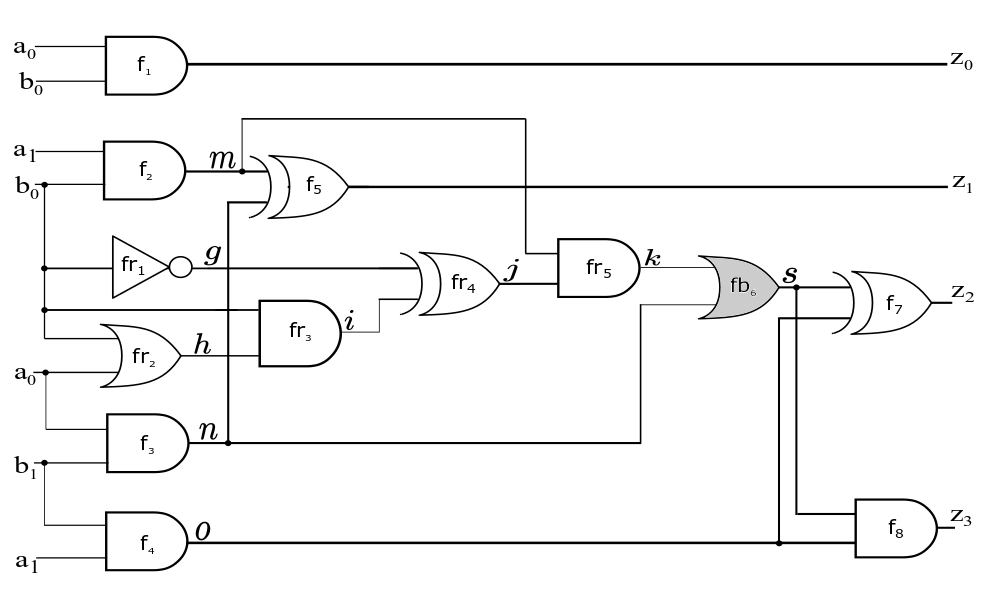
\includegraphics[scale = 0.2]{int_mul_red_b.png}
    \caption{2-bit integer multiplier with a bug at $s$.}
    \label{fig:3mult}
\end{figure}

The \spec is: $f = \sum_{i=0}^{2n-1}
2^iz_i-\sum_{i=0}^{n-1} 2^ia_i\cdot \sum_{i=0}^{n-1} 2^ib_i$.
Verification is done by performing \Grobner Basis reduction, $f
\xrightarrow{J+J_0}_+r$. We find $r = -4\cdot a_0\cdot a_1\cdot
b_0\cdot b_1+4\cdot a_0\cdot b_1$. Since $r \neq 0$, verification
detects the presence of a bug in the design. We will now attempt to
rectify the circuit at an internal net (single-fix
rectification is possible at net $s$ itself!). 
\end{Example}
